\section{Implementierung}\label{sec:Implementierung}\label{secmin:Implementierung}

In einem System, in welchem ein \gls{Multi-User Betrieb} möglich sein soll, ist das Design der Oberfläche und das der einzelnen Benutzerschnittstellen unweigerlich eng miteinander verknüpft. 
Es müssen in der Phase der Implementierung bereits exakte Schnittstellen definiert und strukturierte Oberflächen skizziert worden sein um spätere Korrekturen gering zu halten oder um sie zu vermeiden.

In den folgenden zwei Abschnitten sollen grundlegende Implementierungsgedanken besprochen werden, die mit den Anforderungen an das System in erster Linie nichts zu tun haben. 
Zuerst soll die Art und Weise der Umsetzung der Benutzerschnittstellen und des Designs näher erklärt werden. Danach sollen elementare Datenstrukturen die zum Einsatz kamen und in JSF implementiert wurde näher erläutert werden.

Nach den beiden einführenden Abschnitten wird dem Leser detailiert dargestellt wie die zu bewältigenden Systemanforderungen in JSF umgesetzt wurden. 
Dabei werden Quellcodeausschnitte sowie Diagramme zum Einsatz kommen die dem Leser das Verstehen erleichtern sollen.
Da während allen Phasen der Umsetzung des Projekts auch immer die Modularität des gesamten Systems im Vordergrund stand soll hier nicht kleinlichst genau erklärt werden was im Quellcode steht, sondern darauf eingegangen werden, wie das zu lösende Problem angegangen wurde und schlussendlich welche wichtigen Bausteine zu tragen kamen. 
An dieser Stelle soll außerdem nochmals die Wichtigkeit der oben besprochenen Datenbankmodellierung erwähnt werden. Gründe für die verschiedenen Umsetzungen der Modellierung sollen im Abschnitt der Implementierung dieser Ausarbeitung nicht mehr näher besprochen werden. 
Es wurde jedoch viel Wert darauf gelegt die Schritte der Implementierung gut und verständlich zu formulieren und darzustellen.

\subsection{Benutzerschnittstellen und Oberflächendesign}

Wir haben uns für ein simples und einfach zu verstehendes Oberflächendesign entschieden, welches allerdings den Design Aspekten der \gls{Corporate Identity} (CI) erfüllen sollte. 
Im allgemeinen wird beim Screendesign bestimmten Regeln gefolgt, welche durch das gewählte Gestaltungsraster festgelegt werden.

Hierzu wurden von uns folgende Bereiche festgelegt:
\begin{itemize}
  \item Kopf- oder Bannerbereich mit Logo
  \item Navigationsbereich bzw. Unternavigation
  \item Arbeitsbereich
  \item Impressum/Hinweise
\end{itemize}

Der Hauptaufbau dieser Seiten, auf welche im folgenden näher eingegangen wird, wurden mit Templates, wie es bereits in \prettyref{subsec:Darstellung von Seiteninhalten} angesprochen wurde, umgesetzt.
Der allgemeine Aufbau soll im folgenden besprochen werden, der nachstehende Quellcodeausschnitt zeigt einen Teil des Templates das von uns zur Gestaltung der Seiten verwendet wurde:

% LISTING
% template.xhtml 
	\lstinputlisting[label={lst:templateFacelet},
	caption={Template-Facelet, dass grundelegenden Aufbau der Seite beschreibt},
	frame=tlbr, 
	language=java, 
	breaklines=true, 
	numbers=left, 
	numberstyle=\tiny, 
	stepnumber=1, 
	numbersep=5pt, 
	basicstyle=\small\ttfamily,
	showstringspaces=true,
	keywordstyle=\bfseries\color{lila}, 
	backgroundcolor=\color{lightgrey}]{listings/template.xhtml}

Auffallend ist vor allem der Kopf der Seite, welcher den Wiedererkennungswert (Vrgl. hierzu die \iz{Website der Schillerschule}{\url{http://www.schillerschule-aalen.de}}) ganu im Sinne des \ac{CI}s steigern soll.
Hierzu wurde die Grafik lediglich transparenter gehalten als ihr Original und hat ganz im Stil der Schule die Überschrift erhalten wie in \prettyref{fig:header_KuWaSys} zu sehen ist.

% Header
\begin{figure}[H]
 \begin{center}
   
\includegraphics[scale=0.4]{img/header_KuWaSys.png}
 \end{center}
 \caption[\textbf{KuWaSys: Banner des Systems (Header)}]{KuWaSys: Banner des Systems (Header)}
 \label{fig:header_KuWaSys}
\end{figure}

Die Navigation und deren Unternavigationspunkte sind im linken Bereich der Website angeordnet und unterstützen den User visuell mit Hervorhebungen, wie in \prettyref{fig:navihervorhebung_KuWaSys} dargestellt ist, bei der Arbeit mit dem System.
Nötige Unternavigationspunkte, falls diese vorhanden sind, öffnen sich automatisch beim Klick auf ein übergeordnetes Menüelement, sodass die komplette Menüstruktur handlich und kompakt dargestellt erscheint und mit einem Blick erfasst werden kann.

Der Arbeitsbereich wird in der Mitte der Seite dargestellt, unterhalb des Kopfbereichs und rechts der Navigation. 
Dieser wird abgetrennt durch blaue Balken (links zur Navigation sowie oben zum Kopfbereich) um die Einteilung der Seite für die Benutzer des Systems eindeutig und übersichtlich zu halten.
Jede Interaktion mit dem System wird in diesem Bereich der Website dargestellt. 

% Infobar
\begin{figure}[h]
 \begin{center}
   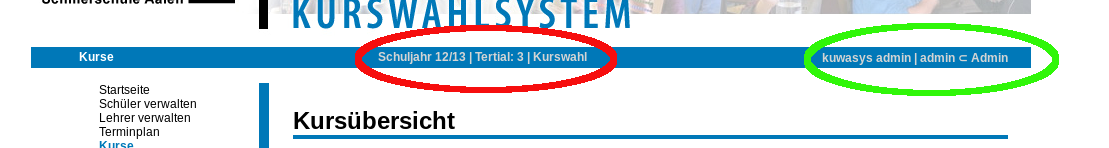
\includegraphics[scale=0.4]{img/informationbar_KuWaSys.png}
 \end{center}
 \caption[\textbf{KuWaSys: Informationsbalken (oberer Bereich)}]{KuWaSys: Informationsbalken (oberer Bereich)}
 \label{fig:infobar_KuWaSys}
\end{figure}

Zur erwähnen ist zudem noch der Trennbalken nach oben welcher zusätzlich als Informationsanzeige für den User verwendet wird und der Fußbereich welcher Informationen zur Website enthält. 
Die obere Anzeige, hier werden Informationen zum User selbst (Voller Name, Username und Rolle im System) und Informationen zum aktuellen Status des Systems (aktuelles Schuljahr und aktuelles Tertial) angezeigt.
Die \prettyref{fig:infobar_KuWaSys} zeigt die genaue Einteilung des Infobalkens oben, rot die Informationen des Systems, grün die Informationen des Users.
Der Fußbereich dient ausschließlich zur weiteren Information beim Besuch der Website welcher in \prettyref{fig:footer_KuWaSys} zu sehen ist.  

Die Hauptfarben des Systems wurden absichtlich blau gewählt um eine gewisse Professionalität sowie Seriösität gegenüber den Benutzern auszustrahlen. Diese ziehen sich kontinuierlich durch das gesamte System

% Navibar
\begin{figure}[H]
 \begin{center}
   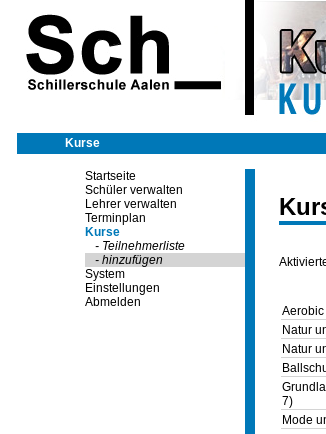
\includegraphics[scale=0.65]{img/navigation_KuWaSys.png}
 \end{center}
 \caption[\textbf{KuWaSys: Navigations und Menüelemente (linker Bereich)}]{KuWaSys: Navigations und Menüelemente (linker Bereich)}
 \label{fig:navihervorhebung_KuWaSys}
\end{figure}

Auf ein Impressum oder auf rechtliche Hinweise konnte bei dieser Art von Website verzichtet werden. 
Erstens handelt es sich hierbei um keine kommerzielle Website, laut \textit{§5} \ac{TMG} wird ein Impressum von 'geschäftsmäßigen Online-Diensten' benötigt, wobei hier die Vorschrift des \textit{§55} \ac{RstV} besagt, dass eine Impressumspflicht nur dann besteht wenn der Inhalt der Website regelmäßig journalistisch-redaktionelle Inhalte online zur Verfügung stellt.
(Gesetzesauszüge sind im Anhang unter \prettyref{subsec:Gesetz} zu finden) 

% Footer
\begin{figure}[h]
 \begin{center}
   
\includegraphics[scale=0.7]{img/footer_KuWaSys.png}
 \end{center}
 \caption[\textbf{KuWaSys: Informationsbalken (unterer Bereich)}]{KuWaSys: Informationsbalken (unterer Bereich)}
 \label{fig:footer_KuWaSys}
\end{figure}

Zur Strukturierung von Seiteninhalten wurden herkömmliche \ac{JSF}-Standardkomponenten verwendet.
Zu den hauptsächlich verwendeten, zählen:
\begin{itemize}
  \item \texttt{<h:outputText>}\\
    Element welches HTML-Text auf der Obefläche ausgibt 
  
  \item \texttt{<h:outputLabel>}\\
    auch normaler Text, allerdings als Beschriftung von Texteingabefeldern
      
  \item \texttt{<h:inputText>}\\
    Element zur Texteingabe, Synonyme für ein HTML \texttt{<input>}-Tag mit type="text"
  
  \item \texttt{<h:inputSecret>}\\
    Element zur verschlüsselten Texteingabe, entspricht \texttt{<input>}-Tag mit type="password"
  
  \item \texttt{<h:commandButton>}\\
    Button in HTML, der Klick löst eine definierte Aktion über eine ManagedBean-Methode aus

  \item \texttt{<h:panelGrid>}\\
    Darstellung einer Tabelle, Synonym für das HTML \texttt{<table>}-Tag. Die Anzahl der Spalten wird über das \texttt{columns}-Attribut festgelegt
  
  \item \texttt{<h:panelGroup>}\\
    Container-Element (mehrere JSF-Tags werden zu einem zusammenfügt)
  
  \item \texttt{<h:message>}\\
    gibt eine Fehlermeldung für die definierte Komponenten aus (\texttt{ErrorStyle}-Attribut über \ac{CSS} steuerbar)
  
  \item \texttt{<h:form>}\\
    stellt ein Formular dar, welches einen POST-Request per HTTP absetzt
  
  \item \texttt{<f:facet>}\\
    Definiert eine Facette (bspw. die Überschrift für eine Tabelle)
\end{itemize}

Außer den eben erwähnten Komponenten gibt es eine Vielzahl anderer bis hin zu selbstdefinierten welche im entwickelten System zum Einsatz kommen. Diese werden allerdings nicht näher betrachtet, da sie für das umgesetzte System irrelevant sind. Selbstverständlich kann zur grafischen Darstellung auch normale \ac{HTML}-Syntax verwendet werden.
Um die Strukturierung des Seitenaufbaus übersichtlich zu halten wird ebenfalls das wohl bereits bekannte Grundlagenwerkezug der Webentwicklung, die \gls{Cascading Style Sheets} (CSS), für die Eigenschaften der Darstellungselemente, eingesetzt.
Vorteile dieser Vorgehensweise der Datenverarbeitung resultiert in einer einheitlichen und damit gut strukturierten Darstellung der betroffenen Websites.

\subsection{Informationsdarstellung und -verarbeitung}

Zunächst soll die Erstellung der Datenbank, für die drei Entities User, Kurs und Notenliste, aufgezeigt werden. Da diese die Grundlage zum Speicher von Daten im System bildet.
In diesem Abschnitt sollen zudem die benutzten Komponenten beschrieben werden die zur Darstellung der Informationen aus der Datenbank verwendet wurden.

\subsubsection{Erstellung der Datenbank}

USER-Tabelle
	CREATE

KURS-Tabelle
	CREATE

NOTENLISTE-Tabelle
	CREATE
	

\subsubsection{Listen und Tabellen}

Eine elementare Datenstrukturen im System sind Listen, welche dem User in Form einer Tabelle im Facelet dargestellt werden.
Die Vorteile dieser Datenstruktur sind die Einfachheit der Datenhaltung sowie der Zugriff auf die Daten und Bereitstellung dieser.

Grundlegend sind drei zu unterscheidende Listen im System implementiert:
\begin{enumerate}
  \item User-Listen (Schüler und Lehrer)
  \item Kurs-Listen
  \item Noten-Listen
\end{enumerate}

Dabei sind die Listen lediglich nach Art des Inhalts zu differenzieren. 
Die für die Benutzeroberfläche relevanten Daten sollen kurz erläutert werden. 

\textbf{Schüler}
\begin{itemize}
  \item ID: Integer, welcher für das Wählen von Kursen und das Vergeben von Noten wichtig ist, da diese einen Fremdschlüssel in der jeweiligen Tabelle darstellt
  \item Vorname und Nachname: String, der den realen Namen des Users wiedergibt
  \item Klasse: String, zur Identifizierung welchem Klassenlehrer ein Schüler zugeordnet ist, bzw wie weit er in seiner Schullaufbahn vorangeschritten ist
  \item Konfession: String, zur Identifizierung des Religionsunterrichts der angeboten werden kann bzw. muss während dem Erstellen eines Kurses. (Näheres in Abschnitt Kurswahl)
\end{itemize}

\textbf{Lehrer}
\begin{itemize}
  \item ID (mit der gleichen Bedeutung wie bei Schülern)
  \item Vorname und Nachname (ebenfalls gleich wie bei Schülern)
  \item Klasse: String, der festlegt, von welcher Klasse ein Lehrer Klassenlehrer ist
\end{itemize}

\textbf{Kurse}
\begin{itemize}
  \item Kursnummer
  \item Kursname
  \item Kursbeschreibung
  \item Teilnehmeranzahl
\end{itemize}

\textbf{Notenlisten}
\begin{itemize}
  \item Schülername
  \item Kursname
  \item Note
  \item Bemerkung
\end{itemize}

Die Implementierung der einzelnen Listen in Java, wurde über Listen vom Typ \texttt{ArrayList<List>} der Klasse \texttt{java.util.ArrayList<E>} umgesetzt. 
Als nächstes soll am Beispiel einer User-Liste gezeigt werden, wie diese im System implementiert wurde.
Hierzu sind zunächst drei Dinge nötig:
\begin{enumerate}
  \item Facelet zur Darstellung
  \item Managed Bean, zum Handling der Daten im Facelet
  \item Klasse, die ein Objekt der jeweiligen Liste, mit den nötigen Attribute, repräsentiert
\end{enumerate}

Die Darstellung der User-Übersicht wird mit Hilfe einer Tabelle umgesetzt.

%% Listing: Facelet mit Tabelle/Liste
	\lstinputlisting[label={lst:userFacelet},
	caption={Facelet einer kompletten User-Übersicht},
	frame=tlbr, 
	language=java, 
	breaklines=true, 
	numbers=left, 
	numberstyle=\tiny, 
	stepnumber=1, 
	numbersep=5pt, 
	basicstyle=\small\ttfamily,
	showstringspaces=true,
	keywordstyle=\bfseries\color{lila}, 
	backgroundcolor=\color{lightgrey}]{listings/users.xhtml}

Das Attribut \texttt{value} der \texttt{<t:dataTable>} referenziert den Inhalt der Liste \texttt{users} in der Backing-Bean \texttt{userBean}. Diese ist jedoch in \texttt{userBean} nur als getter-Methode \texttt{getUsers()} vorhanden und kein Attribut der Klasse.

%% Listing: UserBean
	\lstinputlisting[label={lst:userBean},
	caption={userBean},
	frame=tlbr, 
	language=java, 
	breaklines=true, 
	numbers=left, 
	numberstyle=\tiny, 
	stepnumber=1, 
	numbersep=5pt, 
	basicstyle=\small\ttfamily,
	showstringspaces=true,
	keywordstyle=\bfseries\color{lila}, 
	backgroundcolor=\color{lightgrey}]{listings/list_UserBean.java}

Die Daten werden beim Aufruf von \texttt{userBean.getUsers()} direkt aus der Datenbank geholt. Die Methode \texttt{listUsers()} ist in der Klasse \texttt{DatabaseHandler} implementiert und liefert nach abfrage der Datenbank ein \texttt{ArrayList<User>} Objekt zurück, dass von der oben gezeigten Tabellendeklaration verarbeitet wird.


Die Klasse User, die ein User-Objekt in der Liste darstellt, ist über eine \texttt{Nested Class} realisiert worden. Das bedeutet, dass die User-Klasse keine unabhängige Klasse, sondern in einer anderen Klasse integriert ist. 

Im Beispiel hier ist die Klasse \texttt{User} in der Klasse \texttt{userBean} integriert.

%% Listing: Nested Class
	\lstinputlisting[label={lst:userClass},
	caption={User Klasse als eingebettete Klasse},
	frame=tlbr, 
	language=java, 
	breaklines=true, 
	numbers=left, 
	numberstyle=\tiny, 
	stepnumber=1, 
	numbersep=5pt, 
	basicstyle=\small\ttfamily,
	showstringspaces=true,
	keywordstyle=\bfseries\color{lila}, 
	backgroundcolor=\color{lightgrey}]{listings/User_UserBean.java}
		
\subsubsection{Kurswahl}
Eine der wichtigsten Funktionen des Systems ist der Kurswahldialog für Schüler. Hier hat ein Schüler die volle Übersicht über die ihm zur Wahl stehenden Kurse im Tertial. Eine Übersicht der bereits gewählten Fächerverbünde und weitere Angeben über der Liste der gewählten Kurse zeigen dem Schüler ob seine Wahl ausreichend oder ggf. angepasst werden muss. 
% Kurswahl
\begin{figure}[h]
 \begin{center}
   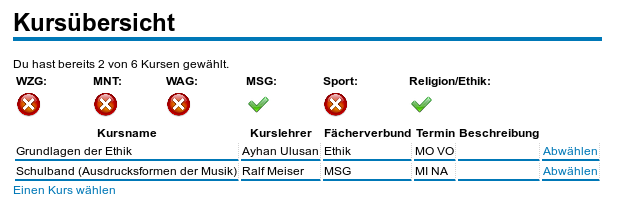
\includegraphics[scale=0.7]{img/kurswahl_KuWaSys.png}
 \end{center}
 \caption[\textbf{KuWaSys: Kurswahldialog für einen Schüler}]{KuWaSys: Kurswahldialog für einen Schüler}
 \label{fig:kurswahl_KuWaSys}
\end{figure}

Auch die Wahl von sich terminlich überschneidenden Kursen wird überprüft und dem Schüler signalisiert. \\Bis ein solcher Konflikt gelöst ist, kann kein weiterer Kurs gewählt werden. 
% Kurswahl_konflikt
\begin{figure}[h]
 \begin{center}
   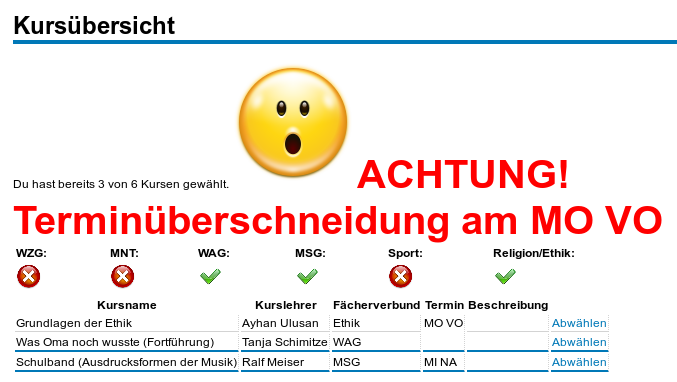
\includegraphics[scale=0.7]{img/kurswahl_konflikt_KuWaSys.png}
 \end{center}
 \caption[\textbf{KuWaSys: Kurswahldialog für einen Schüler bei Terminkonflikt}]{KuWaSys: Kurswahldialog für einen Schüler bei Terminkonflikt}
 \label{fig:kurswahl_konflikt_KuWaSys}
\end{figure}

Am Beispiel der Kurswahl soll nun exemplarisch der Weg von View zu Datenbank (oder umgekehrt) dargestellt werden.
\\ Gewählte und wählbare Kurse werden, wie die oben beschriebenen User in einer Liste gerendert. In diesem Fall kommt jeweils eine Funktion hinzu um einen Kurs zu wählen bzw. abzuwählen. \\Da das Facelet zur Anzeige der Kurse für alle Benutzergruppen notwendig ist, wird beim Rendern abgefragt um welche Art Benutzer es sich handelt und die Seite entsprechend dargestellt.

Um zwischen einem Kreuz und einem Haken für den Status der Wahl eines Fächerverbunds zu untescheiden findet der aus C bekannte ternäre Operator seine Anwendung. Liefert die in der \texttt{courseBean} implementierte Methode \texttt{bundleChosen(String bundle)} den Wert \texttt{true}, wird der Dateiname der Hakengrafik zum Rendern verwendet, andernfalls der der Kreuzgrafik.
%% Listing: courses.xhtml
	\lstinputlisting[label={lst:bundleChosen_courses.xhtml},
	caption={Ausschnitt aus courses.xhtml (1)},
	frame=tlbr, 
	language=java, 
	breaklines=true, 
	numbers=left, 
	numberstyle=\tiny, 
	stepnumber=1, 
	numbersep=5pt, 
	basicstyle=\small\ttfamily,
	showstringspaces=true,
	keywordstyle=\bfseries\color{lila}, 
	backgroundcolor=\color{lightgrey}]{listings/bundleChosen_courses.xhtml}
Ähnlich wird bei der Terminkonfliktprüfung vorgegangen. Die ebenfalls in der der \texttt{courseBean} implementierte Methode \texttt{isDateConflicting()} liefert im Regelfall den Wert '0'. Wird ein Konflikt gefunden, gibt sie den Zeitpunkt als \texttt{String} zurück. Das überraschte Gesicht und der Hinweis, mit dem Rückgabewert werden angezeigt. 
\\ Es ist wichtig, dass nicht einfach gegen die Zahl 0 verglichen wird, sondern gegen die Zeichenkette (einfache Anführungszeichen). Wie wir bei der Präsentation des Systems schmerzlich erfahren mussten, gehen verschiedene Versionen des \texttt{tomcat7} unterschiedlich mit dieser Problematik um. Während auf der im Eclipse eingerichteten Testumgebung die implizite Typenkonvertierung problemlos von statten ging, lieferte das produktive System einen Fehler bei der Typenumwandlung.
%% Listing: courses.xhtml
	\lstinputlisting[label={lst:konflikt_courses.xhtml},
	caption={Ausschnitt aus courses.xhtml (2)},
	frame=tlbr, 
	language=java, 
	breaklines=true, 
	numbers=left, 
	numberstyle=\tiny, 
	stepnumber=1, 
	numbersep=5pt, 
	basicstyle=\small\ttfamily,
	showstringspaces=true,
	keywordstyle=\bfseries\color{lila}, 
	backgroundcolor=\color{lightgrey}]{listings/konflikt_courses.xhtml}	
	
Mittels des \texttt{rendered} Attributes wird abgefragt ob ein Nutzer die Rolle Schüler oder Lehrer besitzt und die jeweilige Aktion zugelassen bzw., falls bereits eine Note gegeben wurde, diese angezeigt. 
%% Listing: courses.xhtml
	\lstinputlisting[label={lst:abwahl_courses.xhtml},
	caption={Ausschnitt aus courses.xhtml (3)},
	frame=tlbr, 
	language=java, 
	breaklines=true, 
	numbers=left, 
	numberstyle=\tiny, 
	stepnumber=1, 
	numbersep=5pt, 
	basicstyle=\small\ttfamily,
	showstringspaces=true,
	keywordstyle=\bfseries\color{lila}, 
	backgroundcolor=\color{lightgrey}]{listings/abwahl_courses.xhtml}
Soll ein Kurs abgewählt werden, wird die Methode \texttt{unAttendCourse} aufgerufen. Dies kann ohne Paramter geschehen, da diese in der analog zur Klasse \texttt{User}, \texttt{Nested}  deklarierten Klasse \texttt{Course} implementiert wurde. Sie ist also Teil eines Kurs-Objekts und hat so direkt Zugriff auf dessen Attribute. 
%% Listing: courses.xhtml
	\lstinputlisting[label={lst:unAttend_CourseBean.java},
	caption={Ausschnitt CourseBean.java},
	frame=tlbr, 
	language=java, 
	breaklines=true, 
	numbers=left, 
	numberstyle=\tiny, 
	stepnumber=1, 
	numbersep=5pt, 
	basicstyle=\small\ttfamily,
	showstringspaces=true,
	keywordstyle=\bfseries\color{lila}, 
	backgroundcolor=\color{lightgrey}]{listings/unAttend_CourseBean.java}
Nachdem eine Instanz der Klasse \texttt{DatabaseHandler} erzeugt wurde, sind deren Methoden verfügbar. \texttt{removeFromGradeList(int userId, int kursId)} führt nun den eigentlichen Zugriff auf die Datebank aus.	
%% Listing: courses.xhtml
	\lstinputlisting[label={lst:removeGrade_DatabaseHandler.java},
	caption={Ausschnitt DatabaseHandler.java},
	frame=tlbr, 
	language=java, 
	breaklines=true, 
	numbers=left, 
	numberstyle=\tiny, 
	stepnumber=1, 
	numbersep=5pt, 
	basicstyle=\small\ttfamily,
	showstringspaces=true,
	keywordstyle=\bfseries\color{lila}, 
	backgroundcolor=\color{lightgrey}]{listings/removeGrade_DatabaseHandler.java}	

\subsection{Import und Export von Datensätzen}
Laut Aufgabenstellung war vom System eine einfache und schnelle Möglichkeit verlangt, Datensätze importieren bzw. exportieren zu können.
Für den Export entschied man sich für CSV- und PDF-Dateien, für den Import sollten nur CSV-Dateien unterstützt werden.
Im folgenden sollen dem Leser beide Mechanismen nähergebracht werden, auf den CSV Import wird in \prettyref{subsec:csvimport} häher eingegangen. 

Im Allgemeinen werden Exports immer über die dafür vorgesehene Buttons gestartet und die dazugehörige Funktion ausgeführt.
Die nötigen Funktionen für die Exports werden in der \texttt{exportBean} zur Verfügung gestellt.
Es sollen nun die Funktionen der Exports näher betrachtet werden.

\subsubsection{CSV-Dateien Export}

Das Exportieren von CSV-Dateien gestaltet sich relativ einfach, da es sich hierbei lediglich um simple Textdateien handelt die mit einem Komma getrennt werden.
Für die Implementierung war es deshalb vorteilhaft, da das Erstellen einer solchen Datei mit einer einfachen Stringverkettung in den Griff zu bekommen ist.

Wird nun per Button eine Funktion der \texttt{exportBean} aufgerufen die CSV-Dateien zu Dowload bereit stellen kann wird eine downloadbare Datei erstellt. Dies geschieht über den \texttt{ContentHeader}, \texttt{ContentType} und die Angabe eines Dateinamens.
Würde man an dieser Stelle die Datei zum Download bereitstellen, würde der User eine leere CSV-Datei erhalten.
Der \prettyref{lstmin:csvExport.java} zeigt stellvertretend für alle CSV-Exports, den klassischen Aufbau einer Exportfunktion.

%% Listing: courses.xhtml
	\lstinputlisting[label={lstmin:csvExport.java},
	caption={Ausschnitt csvExport.java},
	frame=tlbr, 
	language=java, 
	breaklines=true, 
	numbers=left, 
	numberstyle=\tiny, 
	stepnumber=1, 
	numbersep=5pt, 
	basicstyle=\small\ttfamily,
	showstringspaces=true,
	keywordstyle=\bfseries\color{lila}, 
	backgroundcolor=\color{lightgrey}]{listings/csvExport.java}	

Das Befüllen der bisher noch leeren Datei wird mit Hilfe einer Datenbankabfrage und eines \texttt{OutputStreams} umgesetzt.
In diesem Beispiel wird lediglich eine Liste verwendet, welche die nötigen Informationen für die Darstellung, beinhaltet.
Mithilfe einer \texttt{for}-Schleife wird die Liste durchiterriert und wie oben beschrieben per Stringverkettung in die CSV-Datei geschrieben.
Abschließend muss der \texttt{HTTP}-Response noch geschlossen werden
	
\subsubsection{PDF-Dateien Export}

Das Erstellen von PDF-Dateien ist mit Hilfer der \texttt{iText-Klassen} realisiert worden.
Hierzu stellt \texttt{iText} verschiedene Programmierschnittstellen zur Verfügung. Die verwendeten sind hier aufgeführt und werden im Quellcodeausschnitt gezeigt. Auf eine genaue Erklärung wird an diester Stelle verzichtet. Die komplette Dokumentation und das gesamte KnowHow von \texttt{iText} kann in \cite{LowagieB-iText} nachempfunden werden.  

Der Ablauf bis zum Aufruf der Funktion die dem User eine fertig PDF zum Download anbietet ist der gleiche wie er im Abschnitt zuvor (CSV-Dateien) behandelt wurde.
An dieset Stelle soll also gezeigt werden wie die PDFs generiert werden, un zwar am Beispiel des in \prettyref{lstmin:pdfExport.java} gezeigten Beispiels:

%% Listing: courses.xhtml
	\lstinputlisting[label={lstmin:pdfExport.java},
	caption={Ausschnitt pdfExport.java},
	frame=tlbr, 
	language=java, 
	breaklines=true, 
	numbers=left, 
	numberstyle=\tiny, 
	stepnumber=1, 
	numbersep=5pt, 
	basicstyle=\small\ttfamily,
	showstringspaces=true,
	keywordstyle=\bfseries\color{lila}, 
	backgroundcolor=\color{lightgrey}]{listings/pdfExport.java}	
	
Zu Beginn weist die Methode ähnliche Strukturen wie beim CSV-Export auf.
Es werden ebenfalls wieder \texttt{ContentType} etc. angegeben. Über \texttt{Document doc = new Document();} wird ein neues Dokumenten Objekt angelegt. Dieses und der OutputStream bilden den \texttt{PdfWriter}.
Gleich wie beim CSV-Export wird erneut eine Liste mit Daten aus der Datenbank gefüllt und mit einer \texttt{for}-Schleife durchiterriert.
Unter Verwendung von \texttt{iText}-Methoden wird die Gestaltung der PDF-Datei umgesetzt. Im \prettyref{lstmin:pdfExport.java} ist bspw. eine Tabelle umgesetzt worden.

\subsection{Benutzerauthentifizierung}

Einer der elementarsten Vorgänge im System ist der Login-Vorgang. Es handelt sich hierbei um einen Vorgang den jeder Benutzer egal mit welcher Rolle vor der Interkation mit dem System durchlaufen muss. Zur Verifizierung eines Users am System wird sein Kürzel, welches beim Anlegen automatisch aus Vor- und Nachnamen generiert wird, sowie ein Passwort, welches ebenfalls automatisch und randomisiert generiert wird, benötigt. Die Anmeldemaske, welche zugleich auch die Startseite des Kurswahlsystems bildet, kann in \prettyref{fig:login_KuWaSys} angesehen werden. Die Registrierung eines Users am System kann ausschließlich durch den Admin erfolgen.

Für den Vorgang des Logins am System besitzt der Servlet-Container Tomcat 7 eine sehr hilfreiche Funktion, die Konfiguation des \ac{DBCP}s des Apache Commons Projekts (\cite{tomcatDBCP}). 

Wie bereits aus dem \prettyref{subsec:Datenbankmodellierung} bekannt ist, haben wir für unser Datenbank eine zusätzliche Tabelle 'Rolle', die mit der Tabelle 'User' in Relation steht, modelliert. Diese wird nun für die Konfiguration des \ac{DBCP}s benötigt.

% Login
\begin{wrapfigure}[10]{l}{10cm}
 \begin{center}
   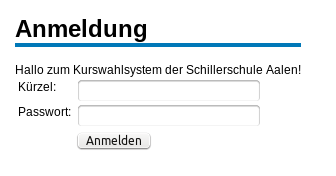
\includegraphics[scale=0.7]{img/login_KuWaSys.png}
 \end{center}
 \caption[\textbf{KuWaSys: Login Maske und Startseite}]{KuWaSys: Login Maske und Startseite}
 \label{fig:login_KuWaSys}
\end{wrapfigure}

% TODO
Der \ac{DBCP} gehört zu einer Art

Aufgrund der Tatsache, dass die Rollen-Tabelle mit der User-Tabelle in einer Beziehung zueinander steht, kann bei der Authentifizierung also genau auf den gewollten User zugegriffen werden. Diese Tatsache machen wir uns auch im weiteren Verlauf der Systemimplementierung zu Nutze, bspw. bei der Generierung von Benutzerdaten (\prettyref{subsec:Daten eines Benutzers}) oder aber um Daten zu manipulieren die mit dem User in Verbindung stehen.

\subsection{Benutzerverwaltung}\label{subsec:Daten eines Benutzers}

\subsubsection{Anlegen von Benutzerdaten}

Das Anlegen eines Benutzers erfordert immer die Informationen über:
\begin{itemize}
  \item Vor- und Nachname
  \item Geburtsdatum
  \item Klasse
  \item Konfession
\end{itemize}

Die Rolle, die ein Benutzer im System erhält, wird durch zwei unterschiedlich Eingabeaufforderungsdesigns umgesetzt. Eines für Lehrer und eines für Schüler. Benutzernamen und Passwörter werden vom System anhand der eingegebenen Informationen automatisch generiert. 

% User anlegen: Schüler
\begin{figure}[H]
 \begin{center}
   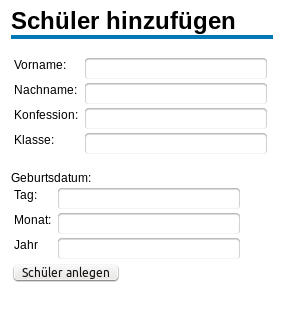
\includegraphics[scale=0.6]{img/UserAnlegen_KuWaSys.png}
 \end{center}
 \caption[\textbf{KuWaSys: User anlegen}]{KuWaSys: User anlegen}
 \label{fig:UserAnlegen_KuWaSys}
\end{figure}


% User anlegen: Lehrer
\begin{figure}[H]
 \begin{center}
   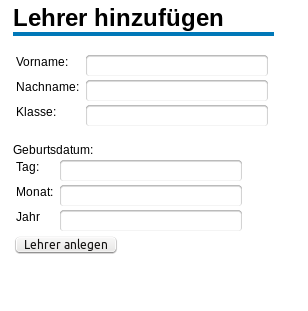
\includegraphics[scale=0.6]{img/LehrerAnlegen_KuWaSys.png}
 \end{center}
 \caption[\textbf{KuWaSys: Lehrer anlegen}]{KuWaSys: Lehrer anlegen}
 \label{fig:LehrerAnlegen_KuWaSys}
\end{figure}

textbf{Sonderfunktion: CSV-Import}
\label{subsec:csvimport}

Eine Besonderheit der Benutzerverwaltung ist der Import von Userdaten über \ac{CSV}-Dateien. Diese Funktion war im Sinner der Projektarbeit nicht gefordert erleichtert aber die Arbeit mit dem System ungemein. Da jedes Jahr, zum Schuljahresbeginn, neue Schüler in das Kursplanungs- und Kurswahlsystem mit aufgenommen werden müssen wäre der Aufwand einzelne Benutzer hinzuzufügen zu groß und langwierig. Außerdem werden CSV-Dateien auch von gängigen Tabellenkalkulationsprogrammen unterstützt.

Als Vorlage für erste Importversuche diente die aktuelle Schülerliste im CSV-Format. Diese enthielt Daten in der Form:
%% Listing: CSV Schüler
	\lstinputlisting[label={lst:schiller_schueler.csv},
	caption={Beispiel einer CSV-Datei mit User Informationen},
	frame=tlbr, 
	language=java, 
	breaklines=true, 
	numbers=left, 
	numberstyle=\tiny, 
	stepnumber=1, 
	numbersep=5pt, 
	basicstyle=\small\ttfamily,
	showstringspaces=true,
	keywordstyle=\bfseries\color{lila}, 
	backgroundcolor=\color{lightgrey}]{listings/schiller_schueler.csv}

Mit Hilfe dieser Datei konnte ein Parser entworfen werden. Umgesetzt wurde der Parser mit der JAVA-Klasse \texttt{StringTokenizer}, um Tokens zu definieren und nach ihnen zu selektieren, und mit der Klasse \texttt{BufferedReader} und \texttt{InputStreamReader}, um die CSV-Datei überhaupt erst einlesen zu können. 

Der \prettyref{lst:ImportBean.java} zeigt die ManagedBean-Klasse \texttt{importBean} mit der Methode \texttt{doImport()}, die den komplettem Parse-Vorgang einer CSV-Datei steuert.
Die wichtigsten Zeilen des Quellcodeausschnitts sollen kurz erläutert werden:
\begin{itemize}
  \item[Zeile]
  \item[08:] Initialisierung der String-Variablen
  \item[23:] Beginn des Parsing-Vorgangs: Solange die CSV-Datei weitere Zeilen enthält
  \item[25:] Initialisierung des StringTokenizers (Zeilen und Angabe des Trennzeichens)
  \item[26:] Zeilenweise Tokens auswählen, solange weitere Tokens existieren
  \item[28:] Switch-Case fängt Integer-Wert der Tokens ab und weist die Werte den richtige Strings zu
  \item[47:] Aufruf der Methode \texttt{addUser} der \texttt{DatabaseHandler}-Klasse, die als Paramter die ausgelesenen Informationen der CSV-Datei enthält und einen neuen User im System anlegt
\end{itemize}

Wie unschwer zu erkennen ist, ist der Parser sehr einfach gestrickt. Es reicht anzugeben welche Trennzeichen zwischen den Daten benutzt werden (Obwohl der Namen CSV als Trennzeichen das Komma suggeriert, können als Trennzeichen zumindest auch Semikoli verwendet werden).
Weiter ist es ausreichend zu wissen wann die CSV-Datei endet und schlussendlich wie die Reihenfolge, der Werte die ausgelesen werden sollen, ist.

%% Listing: CSV Schüler - Parser
	\lstinputlisting[label={lst:ImportBean.java},
	caption={CSV-Datei Parser-Methode},
	frame=tlbr, 
	language=java, 
	breaklines=true, 
	numbers=left, 
	numberstyle=\tiny, 
	stepnumber=1, 
	numbersep=5pt, 
	basicstyle=\small\ttfamily,
	showstringspaces=true,
	keywordstyle=\bfseries\color{lila}, 
	tabsize=2,
	backgroundcolor=\color{lightgrey}]{listings/ImportBean.java}

\subsubsection{Festlegen von Usernamen}

Die Generierung von Usernamen wird einheintlich vom System beim Hinzufügen eines neuen Benutzers gewährleistet.
Ein Usernamen besteht immer aus einer Zeichenkette die wie folgt aufgebaut ist:

\[
\begin{split}
  \text{Username} =\quad & 3\quad \text{Buchstaben des Nachnamens}\\ 
  +\quad & 2 \quad \text{Buchstaben des Vornamens}\\ 
  +\quad & \text{laufende Nummer}
\end{split}
\]

So wird beim Anlegen des Users 'Christian Silfang' im System:

\[
\begin{split}
  \text{SilCh1} &= \quad \text{Sil} \quad (3 \quad \text{Buchstaben des Nachnamens})\\ 
		&+ \quad \text{Ch} \quad (2 \quad \text{Buchstaben des Vornamens})\\ 
		&+ \quad 1 \quad (\text{laufende Nummer})
\end{split}
\]

Im Programmcode wird diese Umwandlung durch herkömmliche \texttt{substring-Methoden} realisiert.
Im nachstehenden \prettyref{lstmin:username} ist dieser Schritt dargestellt. Die Besonderheit bei dieser Funktionalität ist die automatische und fortlaufende Generierung der User-Ziffer. So wird gewährleistet, dass ein Username im System eindeutig ist. Letztendlich steckt dahinter eine Datenbankabfrage, die auf eventuell bestehende Usernamen prüft.
Falls ein Username nun im System vorhanden ist, wird die Nummer erhöht und der Vorgang wird erneut von vorne gestartet. Tritt der Fall ein, dass ein Username im System nicht vorhanden ist, so wird der eben generierte Username für den dazugehörigen User gespeichert. Der Umschaltmechanismus wird dabei durch eine Boolsche Variable \texttt{isCurrentUsername} (Zeile 9) gesteuert.

%% Listing: Username generiert
	\lstinputlisting[label={lstmin:username},
	caption={Usernamen generieren},
	frame=tlbr, 
	language=java, 
	breaklines=true, 
	numbers=left, 
	numberstyle=\tiny, 
	stepnumber=1, 
	numbersep=5pt, 
	basicstyle=\small\ttfamily,
	showstringspaces=true,
	keywordstyle=\bfseries\color{lila}, 
	tabsize=2,
	backgroundcolor=\color{lightgrey}]{listings/usernames_generate.java}


\subsubsection{Generierung von Passwörtern}

Das Generieren von Passwörtern ist sehr simpel umgesetzt. Hierzu wurden einfach Zufallszahlen- und Ziffernfolgen generiert:

%% Listing: Passwort generieren
	\lstinputlisting[label={lstmin:pwd},
	caption={Passwort generieren},
	frame=tlbr, 
	language=java, 
	breaklines=true, 
	numbers=left, 
	numberstyle=\tiny, 
	stepnumber=1, 
	numbersep=5pt, 
	basicstyle=\small\ttfamily,
	showstringspaces=true,
	keywordstyle=\bfseries\color{lila}, 
	tabsize=2,
	backgroundcolor=\color{lightgrey}]{listings/passwort_generate.java}
	
Die Sicherheit der Passwörter ist durchaus gegeben.
Die momentanen Passwörter, haben eine Länge von 7. Ursprünglich waren Längen von 16 Zeichen implementiert. Nach Absprache mit der Schule, wurden diese herunter gekürzt.

\subsection{Kursverwaltung}

Neben dem Anlegen von neuen Benutzern, muss das System auch die Funktionalität besitzen, neue Kurse hinzuzufügen.
Die Schillerschule arbeitet mit sogenannten Fächerverbünden. Fächerverbünde fassen einzelne Kurse in Thematik und Kompetenz zusammen.
Die Fächerverbünde im einzelnen sind:

\begin{itemize}
  \item \ac{MSG}

  \item \ac{WAG}
  
  \item \ac{MNT}
  
  \item \ac{WZG}
\end{itemize}

Gesondert behandelt werden lediglich Religionskurse. Diese werden keinem Verbund zugeordnet sondern sind selbstständig.
Kurse können generell an jedem Wochentag stattfinden. Ein Kurs wird allerdings nur einmal wöchentlich, entweder vormittags oder nachmittags, angeboten.
Genrell ist es auch nur möglich einen Kurs vormittags oder nachmittags zu besuchen, nicht zwei oder mehrere.
Eine Darstellung des Stundenplans einer Kurswahl, ohne Kernfächer, könnte der folgende sein:
\begin{figure}[H]
\centering
\begin{tikzpicture}[x=\daywidth, y=-1cm, node distance=0 cm,outer sep = 0pt]
% Style for Days
\tikzstyle{day}=[draw, rectangle,  minimum height=1cm, minimum width=\daywidth, fill=yellow!20,anchor=south west]
% Style for hours
\tikzstyle{hour}=[draw, rectangle, minimum height=2cm, minimum width=\daywidth, fill=yellow!30,anchor=north east]

% Styles for events
% Dauer Stunden
\tikzstyle{hours}=[rectangle,draw, minimum width=\daywidth, anchor=north west,text centered,text width=5 em]
\tikzstyle{1hour}=[hours,minimum height=2cm, minimum width=\daywidth, anchor=north west,text centered,text width=5 em]

% Style der Fächer
\tikzstyle{Kurs1}=[1hour,fill=red!20]
\tikzstyle{Kurs2}=[1hour,fill=blue!20]
\tikzstyle{Kurs3}=[1hour,fill=blue!10]
\tikzstyle{Kurs4}=[1hour, pattern=north east lines, pattern color=magenta]
\tikzstyle{Kurs5}=[1hour, pattern=north west lines, pattern color=magenta!60!white]s
\tikzstyle{Kurs6}=[1hour, fill=green!10]
\tikzstyle{Pause}=[1hour, fill=yellow!10]

% Positioning Tag/Stunden
\node[day] (mo) at (1,8) {Montag};
\node[day] (di) [right = of mo] {Dienstag};
\node[day] (mi) [right = of di] {Mittwoch};
\node[day] (do) [right = of mi] {Donnerstag};
\node[day] (fr) [right = of do] {Freitag};

\node[hour] (Vormittag) at (1,8) {Vormittag};
\node[hour] (Pause) [below = of Vormittag] {Pause};
\node[hour] (Nachmittag) [below= of Pause] {Nachmittag};

% Position Fächer
\node[Kurs1] at (1,8) {MSG};
\node[Kurs3] at (2,8) {Sport};
\node[Kurs2] at (3,8) {WZG};
\node[Kurs3] at (5,8) {Sport};
\node[Kurs6] at (4,8) {WAG};
\node[Kurs5] at (1,12) {Reli};
\node[Kurs5] at (2,12) {Reli};
\node[Kurs4] at (3,12) {MNT};
\node[Kurs1] at (4,12) {MSG};
\node[Kurs2] at (5,12) {WZG};
\node[Pause] at (1,10) {};
\node[Pause] at (2,10) {};
\node[Pause] at (3,10) {};
\node[Pause] at (4,10) {};
\node[Pause] at (5,10) {};

\end{tikzpicture}
\caption[\textbf{Kursplan der Schillerschule}]{Kursplan der Schillerschule}
\label{fig:Stundenplan}
\end{figure}

\subsubsection{Daten von Kursen}

Der Aufbau eines Kurses im System, wie aus dem ER-Modell in \prettyref{fig:ERModell} entnommen werden kann, besteht im Grunde aus einer Nummer, einem verantwortlichen Lehrer, einer Beschreibung, einem Termin, Information des dazugehörigen Fächerverbunds  und einer Teilnehmeranzahl. Allein mit diesen Information könnte ein Kurs im System dargestelltn werden. Hierbei werden jedoch die restlichen Attribute vernachlässigt. Diese sollen im folgenden näher zur Sprache kommen.  

Da die angebotenen Kurse im System nun verschiedenen Abhängigkeiten haben können und eventuell bestimmte Vorraussetzungen erfüllen können müssen, wurde eine Möglichkeit gesucht diese Kurse möglichst einfach im System abzubilden. 
Einfach bedeutet an dieser Stelle, dass die Darstellung eines Kurses für alle Rollen gleichermaßen zur Verfügung stehen muss und außerdem Interaktionen mit ihnen unterstützt.
Hierbei müssen die oben vernachlässigten Attribute beachtet werden. 

Attribute die hierbei einer Rolle spielen sind: (Vrgl. ER-Modell in \prettyref{subsec:ERModell})
\begin{itemize}
  \item Sportkurs
  \item Konfession (derzeit EV, RK und Ethik)
  \item Pflichtkurse
\end{itemize}

\textbf{Sportkurse}

Hierbei handelt es sich um ein Attribut, also einer Spalte in der Kurs-Tabelle, die den Datentyp \texttt{boolean} besitzt.
Beim Anlegen hat der Lehrer oder der Admin die Möglichkeit dieses Attribut des zu erstellenden Kurses zu setzen, wie es die grüne Markierung in \prettyref{fig:KursAnlegen_KuWaSys} zeigt.

Das anlegen des Sportkurs-Flags in der DB ist trivial und wird daher nicht weiter betrachtet.

Von einer Besonderheit bei Sportkursen kann gesprochen werden wenn zusätzlich die Fächerverbünde und Pflichtkurse mitbetrachtet werden.
Für gewöhnlich wird ein Sportkurs dem Fächerverbund \ac{MSG} zugeordnet. Es kann allerdings vorkommen, dass ein Kurs als Sportkurs angelegt wird, aber keinen Pflichtkurs darstellt.  
Wichtig ist zu beachten das unabhängig vom Fächerverbund eine gewisse Anzahl an Sportkursen besucht werden muss. Ein Schüler kann also gleichzeitig Sportkurse und den Fächerverbund \ac{MSG} abdecken. Eventuell deckt er hierbei noch zusätzlich einen Pflichtkurs ab oder nicht.
Die gleiche Betrachtungsweise gilt auch für Religionskurse. Allerdings weiß man bereits, dass Religionskurse eigenständige Fächerverbünde darstellen.

Beim Anlegen hat der Lehrer oder der Admin die Möglichkeit dieses Attribut des zu erstellenden Kurses zu setzen, wie es die grüne Markierung in \prettyref{fig:KursAnlegen_KuWaSys} zeigt.


\textbf{Religionsunterricht}

Eine richtige Besonderheit stellt das Anlegen eines Religionskurses dar.
Das Anlegen eines Religionskurses (grüne Markierung in \prettyref{fig:KursAnlegen_KuWaSys}) wird über einfach Selectboxen realisiert. Der Inhalt der Selectboxen wird dazu automatisch angelegt. Wie dies gewährleistet wird soll nun näher besprochen werden.

Wie bereits in \prettyref{fig:UserAnlegen_KuWaSys} gezeigt wurde, wird beim Anlegen eines Users im System, eine Konfessionszugehörigkeit beigefügt. Dieses Feld kann vom Admin beliebig ausgefüllt werden. 
Dieser beliebige String wird in die Tabelle 'Kurskonfession' eingetragen und wird später, durch die Auswahl beim Anlegen eines Kurses, als Fremdschlüssel in der 'Kurs'-Tabelle gespeichert.
Der Inhalt der Selectboxen die zur Verfügung stehen, ist also immer komplette Inhalt der Kurskonfession-Tabelle.

Diese Art der Lösung soll in Zukunft alternative Unterrichte, anderer Konfessionen, zulassen können.

% Kurs anlegen
\begin{figure}[H]
 \begin{center}
   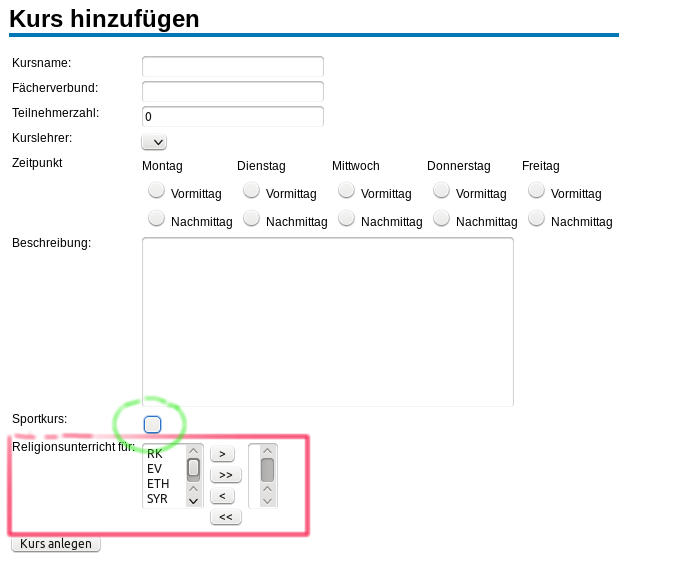
\includegraphics[scale=0.6]{img/KursAnlegen_KuWaSys.png}
 \end{center}
 \caption[\textbf{KuWaSys: Kurs anlegen}]{KuWaSys: Kurs anlegen}
 \label{fig:KursAnlegen_KuWaSys}
\end{figure}

\textbf{Pflichtkurse}

Ähnlich wie bei Sportkursen handelt es sich hierbei um ein Attribut, also ebenfalls einer Spalte in der Kurs-Tabelle, die auch den Datentyp \texttt{boolean} besitzt.
Im Gegesatz zu Sportkursen wird das Pflichtkurs-Flag allerdings nicht beim Anlegen eines Kurses gesetzt. Es kann nur vom Admin bestimmt werden, ob ein Kurs ein Pflichtkurs ist oder nicht. Festlegen kann er dies in der Kursverwaltung in der Phase der Kursplanung.

Die \prettyref{fig:KursVerwalten_KuWaSys} zeigt einen Ausschnitt der Kursverwaltung aus Sicht des Admins.
Der Admin hat die Möglichkeit Kurse zu aktivieren, also den Schülern die Kurse zur Kurswahl zur Verfügung zu stellen oder bereits aktivierte Kurse wieder zu deaktivieren.
Darüberhinaus legt der Admin die Pflichtkurse fest.

% Kurs verwalten
\begin{figure}[H]
 \begin{center}
   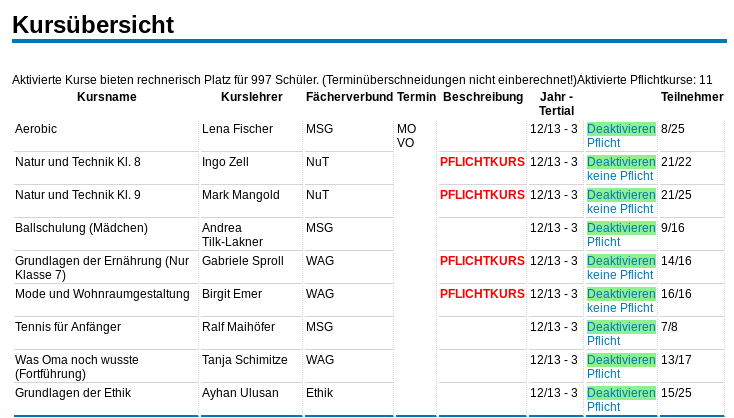
\includegraphics[scale=0.6]{img/KursVerwalten_KuWaSys.png}
 \end{center}
 \caption[\textbf{KuWaSys: Kurse verwalten}]{KuWaSys: Kurse verwalten}
 \label{fig:KursVerwalten_KuWaSys}
\end{figure}
